\chapter{Artificial Neural Networks}
\label{chap:anns}

\begin{quotation}
      ``Men ought to know that from the brain, and from the brain only, arise our pleasures, joy, laughter and jests, as well as our sorrows, pains, griefs, and tears.''
\end{quotation}
\begin{flushright}
      - Hippocrates
\end{flushright}

The human brain is one of the most complicated biological organs in nature. It gives us the ability to think and learn. The field of \acs{ML} has taken a lot of inspiration from the biological brain which lead to the development of \acp{ANN}~\cite{ref:rosenblatt:1958}. \acp{ANN} are used throughout this dissertation as the \textit{model} to be trained using \acp{HH}. The purpose of this chapter is to provide the necessary background information needed on \acp{ANN} and is structured as follows:

\begin{itemize}
      \item \textbf{Section~\ref{sec:anns:bn}} gives background information on the \acs{BN}.

      \item \textbf{Section~\ref{sec:anns:an}} introduces the \acs{AN}. Brief discussions follow on input, \index{weights}weights and \index{biases}biases, \index{net input signal}net input signal, \index{activation function}activation functions, and output.

      \item \textbf{Section~\ref{sec:anns:ann}} introduces the \acs{ANN}. Brief discussions follow on \acs{ANN} architecture, topology, and \acp{FFNN}.

      \item \textbf{Section~\ref{sec:anns:training}} provides details on the training process, \index {supervised learning}supervised learning, training sets, stopping conditions, performance measures and \index{error function}error functions.

      \item \textbf{Section~\ref{sec:anns:summary}} provides a brief summary of the chapter.
\end{itemize}


\index{biological neuron}
\section{Biological Neuron}\label{sec:anns:bn}

This section introduces the \acs{BN} and provides the necessary background information that show how the \acs{BN} has inspired the development of the \acs{AN}.

\begin{figure}[htb]
      \centering
      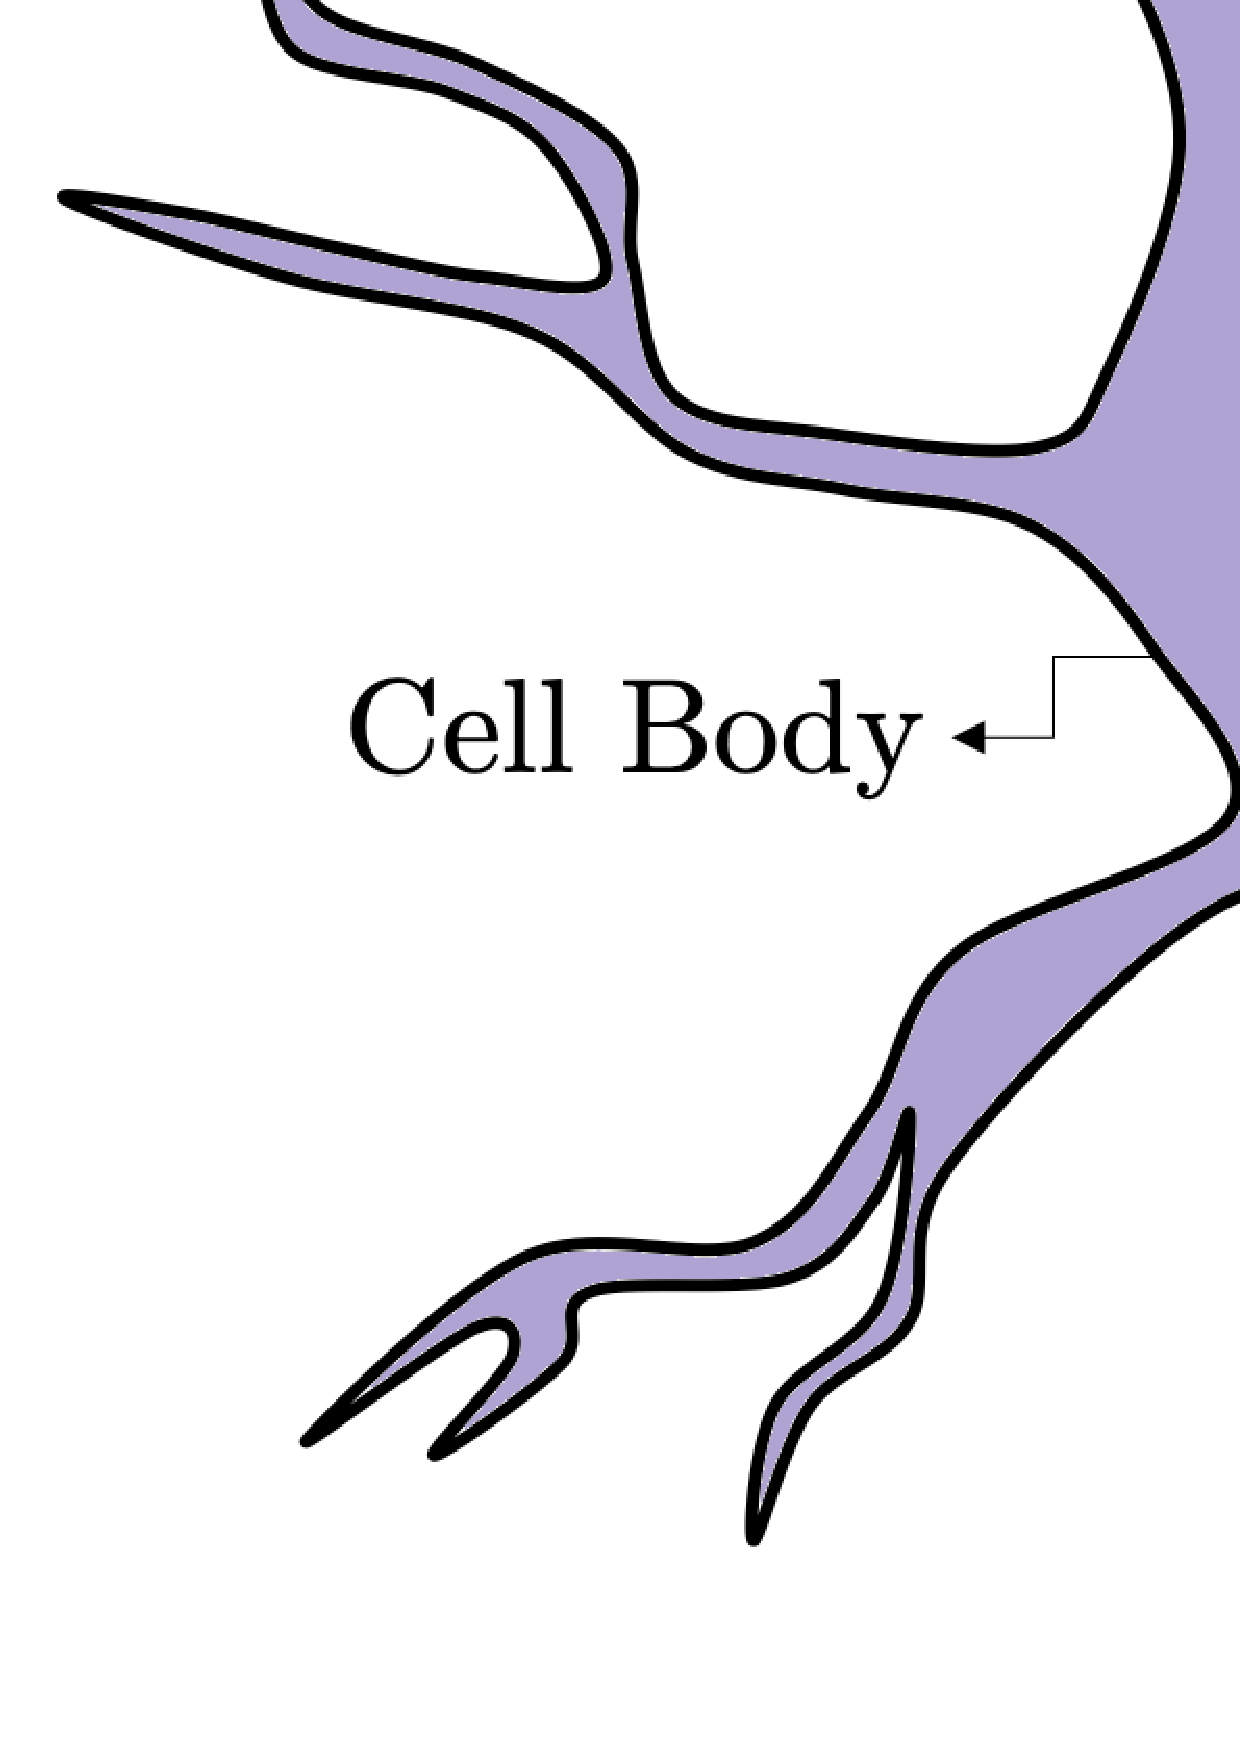
\includegraphics[width=0.95\textwidth]{biological_neuron.pdf}
      \caption[The \index{biological neuron}biological Neuron]{An illustration of the \index{biological neuron}biological Neuron.}
      \label{fig:biological_neuron}
\end{figure}

The biological neural systems are made up of microscopic nerve cells called neurons~\cite{ref:jain:1996}. Figure~\ref{fig:biological_neuron} illustrates a single \acs{BN}. The main components of the \acs{BN} include the cell body, \index{dendrites}\textit{dendrites} and the \index{axon}\textit{axon}. \Acp{NN} are formed through the connections between the \index{axon}axons and \index{dendrites}dendrites of various neurons. This is known as \index{synaptogenesis}\textit{synaptogenesis}~\cite{ref:huttenlocher:1997}. Such a connection is referred to as a \index{synapse}\textit{synapse}. Communication takes place, through the synapse, by electro-chemical pulse and is often referred to as an \textit{activation} or \textit{action potential}.  Communication signals propagate from the \index{dendrites}dendrites, through the cell body to the axon of a neuron, provoking a signal in the post-synaptic neuron~\cite{ref:engelbrecht:2007}. The greater the connection between two neurons, the stronger the communication. Kennedy~\cite{ref:kennedy:2016} defines stronger \index{synapse}synapses as ones that contribute more depolarisation to the neural membrane upon activation than weaker ones. Stronger \index{synapse}synapses have a higher probability of generating an action potential in the post-synaptic neuron. During activation, the pre-synaptic neuron release neurotransmitters that bind to the post-synaptic neuron. The frequent release of these molecules cause the \index{synapse}synapse to grow. Connections that grow over time yield stronger signals (learning), while connections that are weak propagate low intensity signals and vanish over time (forgetting). The ability of synapses to strengthen and weaken over time is known as \index{synaptic plasticity}\textit{synaptic plasticity}~\cite{ref:huttenlocher:1997}.

\index{artificial neuron}
\section{Artificial Neuron}\label{sec:anns:an}

This section introduces the \acs{AN}. Brief discussion follow on the various components that make up the \acs{AN}.

The \acs{AN} implements a non-linear mapping from $\mathbb{R}^{I}$ to
$\mathbb{R}^{T}$, usually in the ranges $[0,1]$ or $[-1,1]$, depending on the
activation function used~\cite{ref:engelbrecht:2007} and is given
as

\begin{equation}
      f_{AN} \colon \mathbb{R}^{I} \to \mathbb{R}^{T}
      \label{eq:an_function_mapping}
\end{equation}

where $f_{AN}$ is the mapping function produced by the \acs{AN}, $I$ is the total number of dimensions of the input in real-number space ($\mathbb{R}$), and $T$ is the total number of dimensions of the target (desired output) in real-number space.

The \acs{AN} implements various components and is illustrated in Figure~\ref{fig:artificial_neuron}.

\begin{figure}[htb]
      \centering
      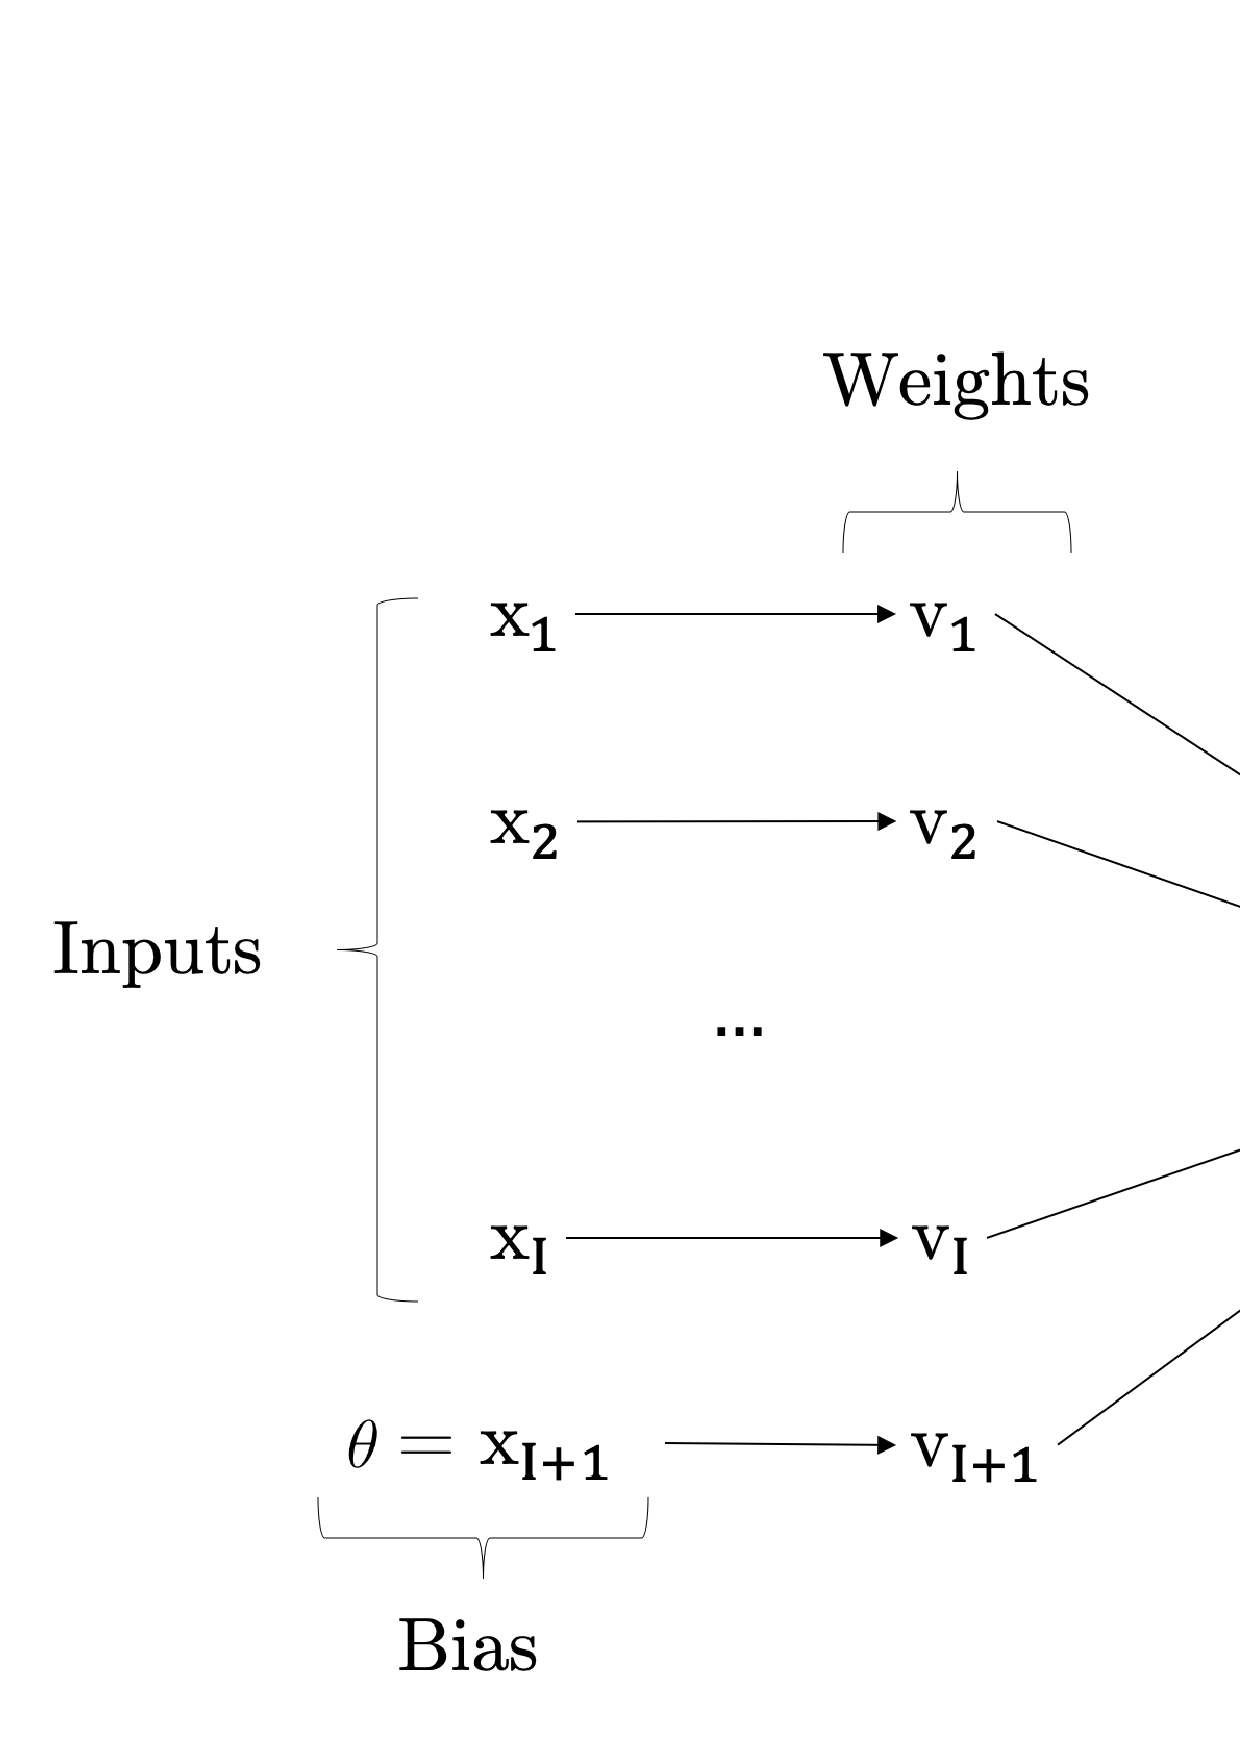
\includegraphics[width=\textwidth]{artificial_neuron.pdf}
      \caption[The \index{artificial neuron}artificial neuron]{An illustration of the \index{artificial neuron}artificial neuron.}
      \label{fig:artificial_neuron}
\end{figure}

Each of the components of the \acs{AN} is inspired by some element of the \acs{BN}. Brief descriptions of these are given as follows:

\begin{itemize}
      \item \textbf{Input:} The input models the activations received from the pre-synaptic neuron or from some environment sensor. Input is represented by the input vector $\boldsymbol{x}$, in Figure~\ref{fig:artificial_neuron}.

      \item \textbf{Weights:} The weights model the \index{synapse}synapses and connection strengths. Weights are represented by the weight vector $\boldsymbol{v}$, in Figure~\ref{fig:artificial_neuron}.

      \item \index{net input signal}\textbf{Net input signal:} The \index{net input signal}net input signal models the net resulting activations from all connected pre-synaptic neurons or environment sensors. The \index{net input signal}net input signal is represented by $net$, in Figure~\ref{fig:artificial_neuron}.

      \item \textbf{Biases:} The biases model a mechanism introduced to influence the strength of the activation (output signal) of the \acs{AN}. The bias is represented by $\theta$, in Figure~\ref{fig:artificial_neuron}.

      \item \index{activation function}\textbf{Activation function:} The activation function models the action potential of the \acs{BN} and is based on the net input signal. The \index{activation function}activation function is represented by $f$, in Figure~\ref{fig:artificial_neuron}.

      \item \textbf{Output:} The output models the activation by the post-synaptic neuron. Output is represented by the output vector $\boldsymbol{y}$, in Figure~\ref{fig:artificial_neuron}.
\end{itemize}

The following sections provide a detailed discussion on each of the above mentioned components.


\subsection{Input}\label{sec:anns:an:input}

Input signals are $I$-dimensional vectors of numerical values that are obtained either through some environment sensor or from other \acp{AN}. Input signals are often referred to as \index{features}\textit{features} or \index{independent variables}\textit{independent variables}~\cite{ref:francis:2001}. Throughout this dissertation, a single input vector is referred to as a \textit{pattern}. Input data must first be pre-processed before it is presented to the \acs{AN}. Input pre-processing techniques are presented in the following sections.


\subsubsection{Input Pre-Processing}\label{sec:anns:an:input:input_pre_processing}

Input pre-processing improves the training process and contributes to the success of the practical application of the \acs{ANN}~\cite{ref:kuzniar:2017}. The primary purpose of input pre-processing is to modify the input data so that it can better match predicted output data. There are many techniques to consider when pre-processing input data. These techniques include methods to encode data to certain formats, to scale to the correct ranges and to deal with incomplete, invalid or irrelevant data. For the purposes of this dissertation, \textit{data encoding} and \textit{normalisation} techniques are considered.


\index{encoding}
\subsubsection{Encoding}\label{sec:anns:an:input:encoding}

For qualitative data, the class labels have to be converted from textual to numerical representations. In general, class labels are encoded as numerical vectors~\cite{ref:brownlee:2017:one-hot}. One such encoding technique is referred to as \index{one-hot encoding}\textit{one-hot encoding}. Harris and Harris~\cite{ref:harris:2010} describe \index{one-hot encoding}one-hot encoding as a group of vector elements where the classes are represented with a single high element (represented by $1$) and all the others low (represented by $0$). Each element $y_k$, where $k$ is the $k$-th element of the encoded vector $\boldsymbol{y}$, uniquely refers to a class. An activation, represented by a value of $1$ at a given index thus represents a class associated with that index.

\index{normalisation}
\subsubsection{Normalisation}\label{sec:anns:an:input:normalisation}

Numerical data must be normalised and scaled appropriately for the \acs{AN}. In general, input data is normalised to a range that is appropriate for the \index{activation function}activation function being used by the \acs{AN}. Normalisation and scaling yields input data that is comparable to the output produced by the \acs{AN}. For the purposes of this dissertation, the \index{min-max scaler}min-max scaler~\cite{ref:al:2006} and the \index{standard score scaler}standard score scaler~\cite{ref:jain:2005} are considered.

\index{min-max scaler}
\subsubsection{Min-Max Scaler}\label{sec:anns:an:input:min_max_scaler}

The \index{min-max scaler}min-max scaler, also called \index{unity-based normalisation}\textit{unity-based normalisation}, scales values to the range $[0,1]$. The \index{min-max scaler}min-max scaler is used as a pre-processing technique for target values when the \index{sigmoid}\textit{sigmoid} \index{activation function} activation function is used. The \index{min-max scaler}min-max scaler is given as

\begin{equation}
      x_{i,p}'  = \frac{x_{i,p} - x_{i_{min}}}{x_{i_{max}} - x_{i_{min}}}
      \label{eq:min_max_scaler}
\end{equation}

where $x_{i,p}^{'}$ is the normalised form of $x_{i,p}$, the $i$-th dimension of the input vector $\boldsymbol{x}_p$, $p \in \{1,2, \dots, P \}$, where $P$ is the total number of input patterns, $x_{i_{min}}$ and $x_{i_{max}}$ are respectfully the minimum and maximum values of the $i$-th dimension for all input vectors $\boldsymbol{x}_p$.

\index{standard score scaler}
\subsubsection{Standard Score Scaler}\label{sec:anns:an:input:standard_score_scaler}

The \index{standard score scaler}standard score scaler, also known as the \index{z-score scaler}\textit{z-score scaler}, scales values by subtracting the mean and scaling to the unit variance of each dimension $i$ for all input patterns $\boldsymbol{x}_p, p \in \{1,2, \dots, P\}$. The \index{standard score scaler}standard score scaler is used as a pre-processing technique for target values when the \index{hyperbolic tangent}\textit{hyperbolic tangent} \index{activation function}activation function\index{activation function} is used. The \index{standard score scaler}standard score scaler is given as

\begin{equation}
      x_{i,p}^{'} = \frac{x_{i,p} - \mu_i}{\sigma^2_i}
      \label{eq:standard_score_scaler}
\end{equation}

where $\mu_i$ and $\sigma^2_i$ are respectfully the mean and unit variance of the $i$-th dimension of all input vectors $\boldsymbol{x}_p$.

\subsection{Weights}\label{sec:anns:an:weights}

The connection strength that synapses in the \acs{BN} have is modelled in the \acs{AN} as weight vectors of numerical values associated with each dimension of the input. Weights can either dampen or strengthen the input by some negative or positive numerical value. Changes in the weight associated with a feature changes the influence that that particular feature has on the predicted output. Finding the correct value for each weight, such that the \acs{AN} yields optimal output, is an optimisation problem~\cite{ref:thierens:1993}. Research has shown that weight initialisation plays an important role in the efficient training of \acp{ANN}~\cite{ref:thimm:1995}.

\subsubsection{Weight Initialisation}\label{sec:anns:an:weights:initialisation}

Weight initialisation is the process by which candidate solutions (represented by the weights of the \acs{AN}) to the problem are ``placed'' in the search space. Weight initialisation influences the speed of convergence, the probability of convergence and the generalisation capabilities of \acp{ANN}~\cite{ref:fernandez:2001}. Finding the optimal initialisation values for weights is non-trivial and can be seen as another optimisation problem~\cite{ref:de:2016, ref:erdogmus:2003, ref:yam:2000}.

Weight initialisation is dependent on the \index{activation function}activation function used. If weights are initialised as values that are too small, the vanishing gradients problem can occur~\cite{ref:hanin:2018}. If weights are initialised as values that are too big, output of the activation function would not be in the active range. This leads to unit saturation, and exploding gradients can occur~\cite{ref:hanin:2018}.

Many different weight initialisation techniques have been developed~\cite{ref:erdogmus:2003}. For the purposes of this dissertation, focus is put on \index{random uniform sampling}random uniform sampling, \index{Glorot uniform sampling}\textit{Glorot uniform (Xavier)} sampling and \index{Glorot normal sampling}\textit{Glorot normal} sampling~\cite{ref:glorot:2010}. Brief discussions on each of these weight initialisation techniques are presented as follows.

\index{random uniform sampling}
\subsubsection{Random Uniform Sampling}\label{sec:anns:an:weights:random_uniform_sampling}

\index{random uniform sampling}Random uniform sampling initialises weights uniformly in the range $[\omega_{min}, \omega_{max}]$, written as $\omega_{i} \sim \textit{U} (\omega_{min}, \omega_{max})$, where the $\omega_{min}$ and $\omega_{max}$ are respectfully the lower and upper bounds of the uniform distribution. Suggested parameter values are $(-1, 1)$ or $(-0.5, 0.5)$~\cite{ref:nguyen:1990}.


\index{Glorot uniform sampling}
\subsubsection{Glorot Uniform Sampling}\label{sec:anns:an:weights:glorot_uniform_sampling}

\index{Glorot uniform sampling}Glorot uniform sampling is a specialisation of \index{random uniform sampling}random uniform sampling, whereby $\omega_{i} = \sqrt{\frac{6}{fanin + fanout}}$ and $fanin$ is the number of input neurons to the weight vector and $fanout$ is the number of output neurons from the weight vector.

\index{Glorot normal sampling}
\subsubsection{Glorot Normal Sampling}\label{sec:anns:an:weights:glorot_normal_sampling}

\index{Glorot normal sampling}Glorot normal sampling initialises weights by sampling from a truncated normal distribution centred on a mean of $0$ and with $\sigma = \sqrt{\frac{2}{I + K}}$, where $\sigma$ is the standard deviation of the distribution. $I$ and $K$ are respectfully the number of input and output units in the weight vector. \index{Glorot normal sampling}Glorot normal sampling has been shown to decrease training time~\cite{ref:glorot:2010}.


\index{net input signal}
\subsection{Net Input Signal}\label{sec:anns:an:net_input}

\acp{AN} accumulate the net resulting input signal from all input dimensions into a value called the \index{net input signal}\textit{net input signal}, expressed as $net$. This signal is passed to the \index{activation function}activation function, which provokes an artificial action potential in the \acs{AN}.

A common way by which the \index{net input signal}net input signal is calculated is by means of \acp{SU}~\cite{ref:engelbrecht:2007}, which compute the \index{net input signal}net input signal as the weighted sum of all input signals and is given as

\begin{equation}
      net = \sum_{i=1}^{I}{x_{i}v_{i}}
      \label{eq:summation_units}
\end{equation}

where $x_{i}$ is the $i$-th dimension of the input vector $\boldsymbol{x}$, and $v_{i}$ is the $i$-th dimension of the weight vector $\boldsymbol{v}$, associated with the given input dimension.


\subsection{Biases}\label{sec:anns:an:biases}

A bias/threshold term $\theta$ is introduced to help translate the output of the \index{activation function}activation function~\cite{ref:benitez:1997}. The value of $\theta$ can be learned during the training process along with the weights of the \acs{ANN}. In order to simplify equations, the input and weight vectors are augmented such that the input and hidden layers have an additional neuron/unit, called the \textit{bias unit}~\cite{ref:engelbrecht:2007}. The net input signal can then be rewritten to consider the bias unit, leading to an augmented net input signal.


\subsubsection{Augmented Net Input Signal}\label{sec:anns:an:biases:augmented_net_input_signal}

The augmented net input signal, that includes the bias unit, has the form $net^{'} = net - \theta$, with $\theta = x_{i+1}v_{i+1}$. A constant value $x_{i+1} = -1$ can be used, meaning that the weight associated with the bias unit, $v_{i+1}$, is optimised along with the other weights during the optimisation process. The net input signal, as given in Equation~\eqref{eq:summation_units}, then changes as

\begin{equation}
      \begin{split}
            net{'} & = net - \theta \\
            & = \sum_{i=1}^{I} x_i v_i - \theta\\
            & = \sum_{i=1}^{I} x_i v_i + x_{i+1} v_{i+1} \\
            & = \sum_{i=1}^{I+1} x_i v_i
            \label{eq:augmented_vectors}
      \end{split}
\end{equation}


\subsection{Activation Functions}\label{sec:anns:an:act_functions}

An \index{activation function}activation function is used to model the action potential of the \acs{AN}~\cite{ref:ziv:1994, ref:hodgkin:1952}. The \index{activation function}activation function takes as a parameter, the augmented \index{net input signal}net input signal. When the output produced by the activation function surpasses some threshold value $\tau$, we consider that neuron to have ``fired'' an output signal. \index{activation function}Activation functions thus model \textit{phase shift}. In the context of classification problems, \index{activation function}activation functions form decision boundaries between classes. In the context of regression problems, \index{activation function}activation functions try to approximate some function that maps the input data to some target data.

In general, activation functions produce a non-linear mapping of $\mathbb{R}^{I}$ to the range $[0,1]$ or $[-1,1]$ as shown in Equations~\eqref{eq:an_function_mapping_0_1} and~\eqref{eq:an_function_mapping_minus_1_1} below.

\begin{equation}
      f_{AN}: \mathbb{R}^{I} \rightarrow [0,1]
      \label{eq:an_function_mapping_0_1}
\end{equation}

\begin{equation}
      f_{AN}: \mathbb{R}^{I} \rightarrow [-1,1]
      \label{eq:an_function_mapping_minus_1_1}
\end{equation}

Many different \index{activation function}activation functions have been developed~\cite{ref:karlik:2011}. For the purposes of this dissertation, focus is put on the \acf{ReLU}~\cite{ref:jarrett:2009, ref:nair:2010}, the \acf{LReLU}~\cite{ref:maas:2013}, the \index{sigmoid}sigmoid~\cite{ref:lecun:1988} and the \index{hyperbolic tangent}hyperbolic tangent~\cite{ref:lin:2008} \index{activation function}activation functions.


\subsubsection{Rectified Linear Unit}\label{sec:anns:an:act_functions:relu}

The \acf{ReLU} \index{activation function}activation function is an \index{activation function}activation function defined in the positive part of its argument and is given as

\begin{equation}
      f(x) = x^{+} = \max(0,x)
      \label{eq:relu}
\end{equation}

An advantage of \acs{ReLU} is that it is not susceptible to the \index{vanishing gradients problem}vanishing gradients problem~\cite{ref:xu:2015} which occurs when gradients in the first layers of a multi-layer \acs{ANN} approach zero, and have no effect on the training process.


\subsubsection{Leaky Rectified Linear Unit}\label{sec:anns:an:act_functions:leaky_relu}

The \acf{LReLU} \index{activation function}activation function is a variant of the \acs{ReLU} \index{activation function}activation function that avoids zero gradients in the negative part of its argument by introducing a scaling parameter, $\alpha > 0$~\cite{ref:xu:2015}. Similar to \acs{ReLU}, \acs{LReLU} is not susceptible to the \index{vanishing gradients problem}vanishing gradients problem. However, \acs{LReLU} does not suffer from the \index{dying ReLU problem}dying \acs{ReLU} problem~\cite{ref:trottier:2017}, which occurs when the neurons that use \acs{ReLU} \index{activation function}activation functions become \textit{inactive} and only output $0$ due to a negative net input signal. The \acs{LReLU} \index{activation function}activation function is given as

\begin{equation}
      f_{AN}(net - \theta) =
      \begin{cases}
            net - \theta         & \text{if $net \geq \theta $} \\
            \alpha(net - \theta) & \text{otherwise}             \\
      \end{cases}
      \label{eq:leaky_relu}
\end{equation}

By introducing a parameter $\alpha > 0$, negative \index{net input signal}net input signals will still yield non-zero activations, resulting in non-zero gradients and avoiding gradient saturation. Non-zero gradients are required by some heuristics such as \acs{SGD} in order to be able to effectively train \acp{ANN}~\cite{ref:hanin:2018}. An illustration of \acs{LReLU} with various values for $\alpha$ and $\theta = 0$ is given in Figure~\ref{fig:anns:activation_functions:leaky_relu}.

\begin{figure}[htb]
      \centering
      \includegraphics[width=0.75\textwidth]{lrelu.pdf}
      \caption[The \acs{LReLU} \index{activation function}activation function]{An illustration of the \acs{LReLU} \index{activation function}activation function with various values for $\alpha$ and $\theta = 0$.}
      \label{fig:anns:activation_functions:leaky_relu}
\end{figure}

\subsubsection{Sigmoid}\label{sec:anns:an:act_functions:sigmoid}

The \index{sigmoid}sigmoid activation is the continuous differentiable approximation of the step function, which was used in the original perceptron model developed by~\citeauthor{ref:rosenblatt:1957}~\cite{ref:rosenblatt:1957}, and yields output in the range $(0, 1)$. The \index{sigmoid}sigmoid \index{activation function}activation function is given as

\begin{equation}
      f_{AN}(net - \theta) = \frac{1}{1+e^{-\lambda(net - \theta)}}
      \label{eq:sigmoid}
\end{equation}

where $\lambda$ is a control parameter that controls the steepness of the sigmoid activation function and is usually set to $\lambda = 1$. An illustration of the \index{sigmoid}sigmoid \index{activation function}activation function with various values for $\lambda$ and $\theta = 0$ is given in Figure~\ref{fig:anns:activation_functions:sigmoid}.

\begin{figure}[htb]
      \centering
      \includegraphics[width=0.75\textwidth]{sigmoid.pdf}
      \caption[The \index{sigmoid}sigmoid \index{activation function}activation function]{An illustration of the \index{sigmoid}sigmoid \index{activation function}activation function with various values for $\lambda$ and $\theta = 0$.}
      \label{fig:anns:activation_functions:sigmoid}
\end{figure}

\subsubsection{Hyperbolic Tangent}\label{sec:anns:an:act_functions:tanh}

The \index{hyperbolic tangent}hyperbolic tangent \index{activation function}activation function has a similar shape to that of the \index{sigmoid}sigmoid \index{activation function}activation function, but yields output in the range $(-1, 1)$. The \index{hyperbolic tangent}hyperbolic tangent \index{activation function}activation function is given as

\begin{equation}
      f_{AN}(net - \theta) = \frac{e^{\lambda(net - \theta)}-e^{-\lambda(net - \theta)}}{e^{\lambda(net - \theta)}+e^{-\lambda(net - \theta)}}
      \label{eq:hyperbolic_tangent}
\end{equation}

An illustration of the \index{hyperbolic tangent}hyperbolic tangent \index{activation function}activation function with various values for $\lambda$ and $\theta = 0$ is given in Figure~\ref{fig:anns:activation_functions:hyperbolic_tangent}.


\begin{figure}[htb]
      \centering
      \includegraphics[width=0.75\textwidth]{tanh.pdf}
      \caption[The \index{hyperbolic tangent}hyperbolic tangent \index{activation function}activation function]{An illustration of the \index{hyperbolic tangent}hyperbolic tangent \index{activation function}activation function with various values for $\lambda$ and $\theta = 0$.}
      \label{fig:anns:activation_functions:hyperbolic_tangent}
\end{figure}


\subsection{Output}\label{sec:anns:an:output}

Output signals are numerical values that represent the output of the \acs{AN}'s \index{activation function}activation function. Output signals are often referred to as \textit{predictions}. Output values need to be post-processed to ensure the practical application of the \acs{AN}.

\subsubsection{Output Post-Processing}\label{sec:anns:an:output:output_post_processing}

Output post-processing converts output values to ranges that better match that of the target values. The post-processing techniques that are applicable depend on the type of problem (regression or classification), pre-processing techniques used, as well as the \index{activation function}activation function used. For the purposes of this dissertation, data decoding, normalisation and
re-scaling techniques are considered.


\subsubsection{Decoding}\label{sec:anns:an:output:decoding}

Data decoding refers to the process of undoing the encoding process. For min-max scaling, data is converted back to the range $(x_{min}, x_{max})$. In the context of an \acs{AN}, binary logistic regression problems map the output to the positive or negative class, usually separating the class decision boundary using a threshold value $\tau$. In the context of multiple \acp{AN}' output, the output is a vector of numerical values. The one-hot encoded output is then decoded by mapping the index of the output vector that yields the highest activation (argmax) to its associated class.

\subsubsection{Softmax}\label{sec:anns:an:output:softmax}

The \index{softmax}softmax function, also known as the \index{softargmax}\textit{softargmax}~\cite[p.~184]{ref:goodfellow:2016} or \index{normalised exponential function}\textit{normalised exponential function}~\cite{ref:bishop:2006} is a generalisation of the logistic function that converts a $K$-dimensional output vector $\boldsymbol{y}$ into a $K$-dimensional output vector $\boldsymbol{y^{'}}$ where each element $y^{'}_k$ is in the range $(0,1)$ and all elements sum up to $1$ as is shown in Equation~\eqref{eq:sum_after_softmax} below.

\begin{equation}
      \boldsymbol{y^{'}} \colon \mathbb{R}^{K} \to \left\{\boldsymbol{y^{'}} \in \mathbb{R}^{K} \vert y^{'}_k \in (0,1), \sum_{k=1}^{K} y_k = 1\right\}
      \label{eq:sum_after_softmax}
\end{equation}

The softmax function is then given as

\begin{equation}
      y^{'}_k = \frac{e^{y_k}}{\sum_{k = 1}^{K}e^{y_k}}
      \label{eq:softmax}
\end{equation}


\subsubsection{Argmax}\label{sec:anns:an:output:argmax}

The \index{argmax}argmax function is similar to the \index{softmax}softmax function, with the difference that the element $y_k, k \in \{1,2, \dots, K\}$ with the highest output value is set to $1$ and the rest are set to $0$. All elements still sum to $1$, but the activation is only observed at index $k$ where the activation is $1$. The \index{argmax}argmax function is given as

\begin{equation}
      y^{'}_k =
      \begin{cases}
            1 & \text{if $y_k = \max(y_1, y_2, \dots, y_K)$} \\
            0 & \text{otherwise}
            \label{eq:argmax}
      \end{cases}
\end{equation}

Figure~\ref{fig:anns:activation_functions:softmax_argmax} illustrates the comparison of transformations of the output vector $\boldsymbol{y}$, where the \index{sigmoid}sigmoid, the \index{softmax}softmax and the \index{argmax}argmax \index{activation function}activation functions are used.


\begin{figure}[htb]
      \centering
      \includegraphics[width=0.75\textwidth]{output_modifiers.pdf}
      \caption[The results of \index{softmax}softmax and \index{argmax}argmax]{An illustration of \index{softmax}softmax and \index{argmax}argmax applied after the \index{sigmoid}sigmoid \index{activation function}activation function.}
      \label{fig:anns:activation_functions:softmax_argmax}
\end{figure}


\section{Artificial Neural Network} \label{sec:anns:ann}

Multiple \acp{AN} can be organised and used together forming a ``network'' of \acp{AN} referred to as an \acf{ANN}. This section presents \acp{ANN} and discussions follow on their applications, architecture, and topologies. Specific reference is made to \acf{FFNN}, a specific type of \acs{AN} used in this dissertation.

\subsection{Applications} \label{sec:anns:anns:applications}

\acp{ANN} are inspired by the biological brain. Our brains model biological neural networks with neuron counts in the hundreds of billions and synapse counts in the trillions. To emulate the computational capability of the human brain is not yet possible on modern day hardware.~\citeauthor{ref:sandberg:2008}~\cite{ref:sandberg:2008} approximates a computational requirement of 256 000 terabytes/s to emulate the entire brain. Despite our shortage in hardware capabilities, \acp{ANN} have been successfully applied to a range of problem classes.~\citeauthor{ref:engelbrecht:2007}~\cite{ref:engelbrecht:2007} summarises some common problems that are solved using \acp{ANN} and can be listed as follows:

\begin{itemize}
      \item \textbf{Classification}: Predicting the class of an input vector~\cite{ref:khan:2001}.

      \item \textbf{Pattern Matching}: Producing closely associated patterns based on an input vector~\cite{ref:cannady:1998, ref:kumar:1994}.

      \item \textbf{Pattern Completion}: Completing the missing parts of an input vector~\cite{ref:dayhoff:2001}.

      \item \textbf{Optimisation}: Producing optimal values of parameters in a optimisation problems~\cite{ref:specht:1991}.

      \item \textbf{Data Mining}: Feature discovery in large datasets~\cite{ref:singh:2009}.
\end{itemize}

The composition of \acp{AN} in an \acs{ANN} is expressed as the \textit{architecture} and \textit{topology} of the \acs{AN}. The exact composition to use depends on the problem being solved.

\subsection{Architecture} \label{sec:anns:anns:architecture}

The architecture of the \acs{ANN} refers to the way in which \acp{AN} are organised. \acp{ANN} can be organised in layers where a single layer can contain multiple \acp{AN}. Generally, each layer makes use of the same \index{activation function}activation function. Output from one layer is propagated as input to the next layer. This dissertation focuses on the simplest architecture, containing three particular layers, including the input, hidden and output layers. \acp{ANN} with this type of architecture are usually referred to as \textit{shallow} \acp{NN}. A description of each layer is given as follows.

\subsubsection{Input Layer}\label{sec:anns:anns:architecture:input}

The input layer contains the input data to the \acs{ANN}. Since the input layer simply provides the input data, some literature do not consider the input layer as an actual part of the \acs{ANN}~\cite{ref:engelbrecht:2007}.

\subsubsection{Hidden Layer}\label{sec:anns:anns:architecture:hidden}

The hidden layer contains a collection of ``hidden'' \acp{AN}, also referred to as \textit{hidden units} or \textit{nodes}. Hidden units are used if the target data is not linearly separable~\cite{ref:engelbrecht:2007}. It has been shown that \acp{ANN} that incorporate monotonically increasing differentiable \index{activation function}activation functions can approximate any continuous function with just one hidden layer, given that the hidden layer has enough hidden units~\cite{ref:hornik:1989}.

\subsubsection{Output Layer}\label{sec:anns:anns:architecture:output}

The output layer contains the final activations or the predictions of the \acs{ANN}. These outputs can be used to measure the performance of the \acs{ANN}.


\subsection{Topology}
\label{sec:anns:anns:topology}

The topology of the \acs{ANN} refers to the way that layers of \acp{AN} are connected to each other. There are many different topologies~\cite{ref:miikkulainen:2010}. For the purposes of this dissertation focus is put on a \index{fully connected topology}\textit{fully connected} topology where each \acs{AN} in one layer is connected to all \acp{AN} in the next, without any cycles~\cite{ref:zell:1994}.


\subsection{Feedforward Neural Networks}\label{sec:anns:anns:ffnns}

\acp{FFNN} were the first and simplest type of \acp{ANN} developed~\cite{ref:schmidhuber:2015} and implement input, hidden and output layers by arranging them in sequential order. Furthermore, \acp{FFNN} implement \index{fully connected topology}fully connected topologies. In \acp{FFNN}, information moves forward, in one direction, from the input nodes, through the hidden nodes and finally to the output nodes. Depending on the optimisation algorithm used, error correction information can be propagated backwards through the network. An illustration of a \acs{FFNN} is given in Figure~\ref{fig:ffnn} below.

\begin{figure}[htb]
      \centering
      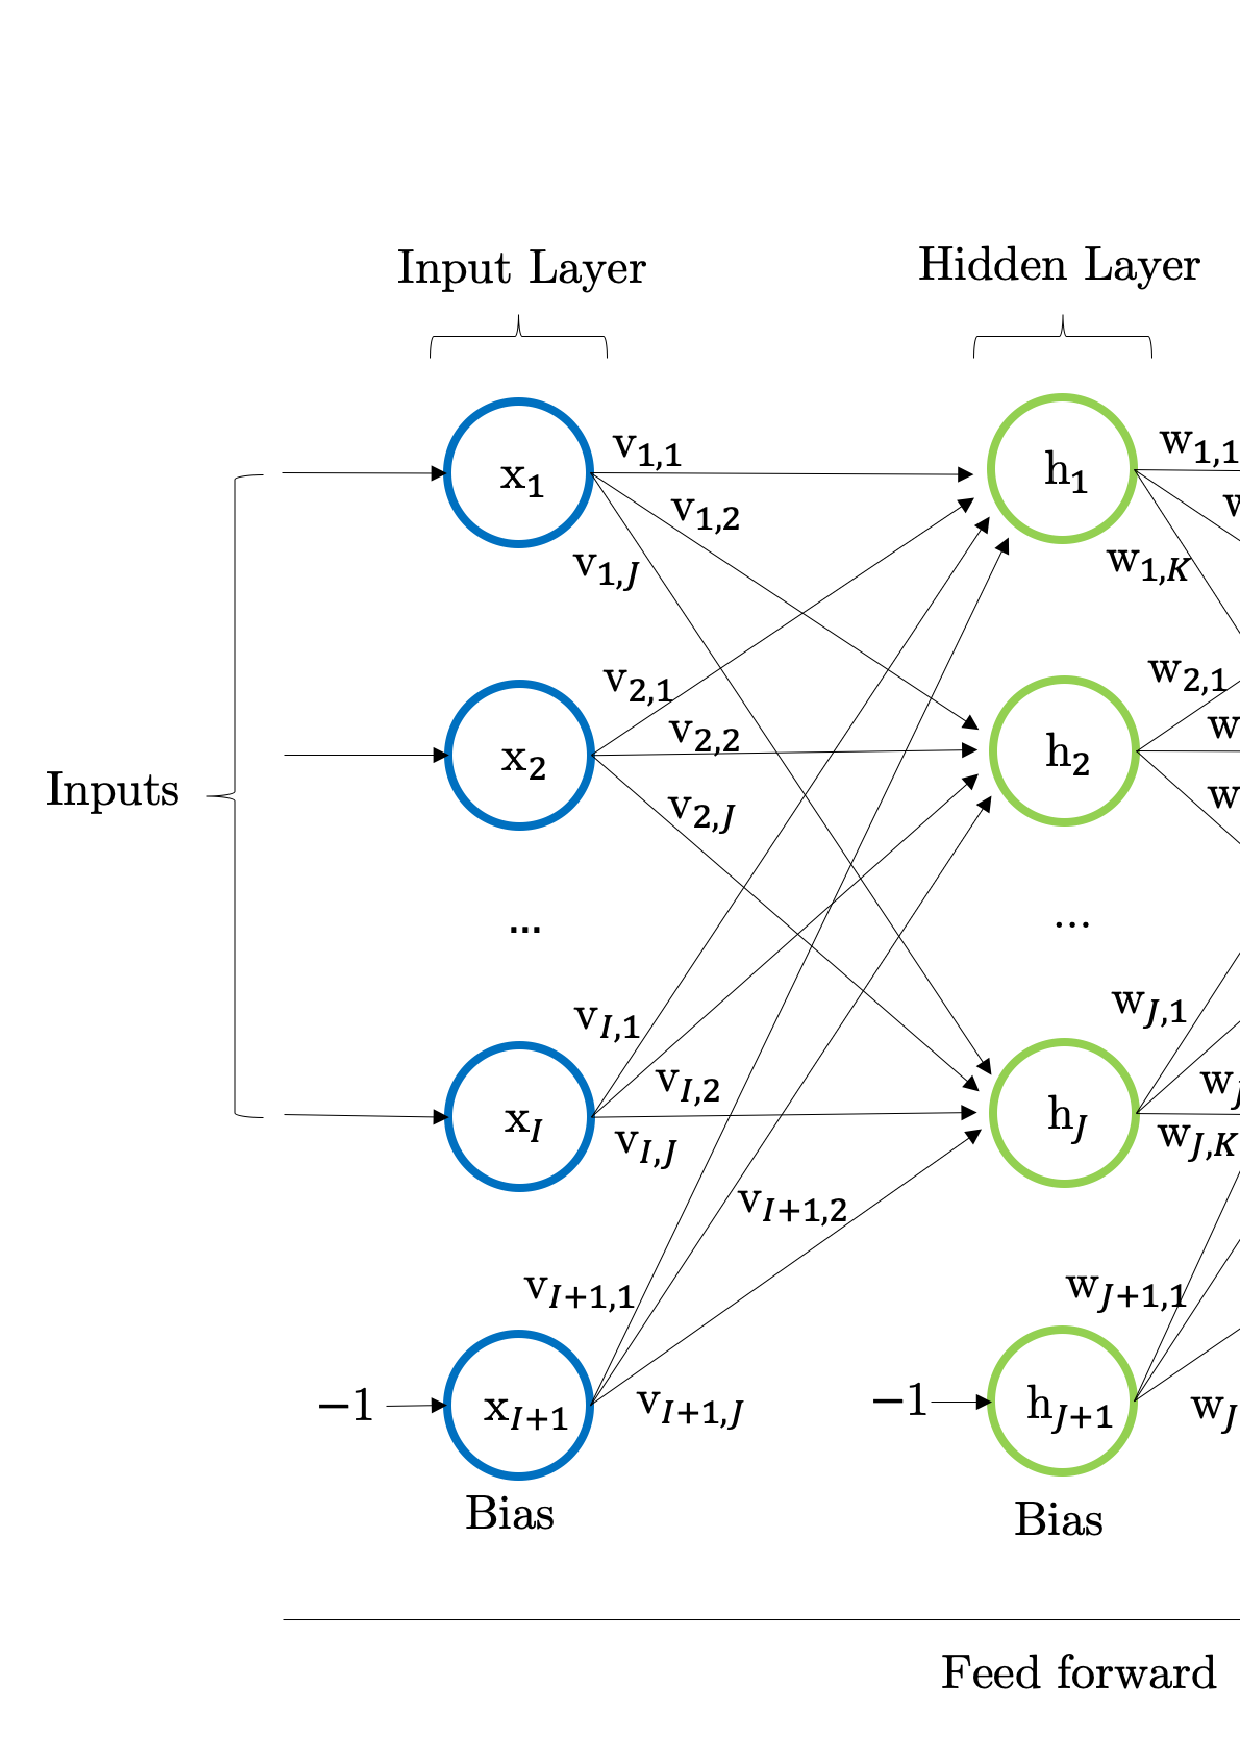
\includegraphics[width=0.98\textwidth]{feedforward_neural_network.pdf}
      \caption[A \index{feedforward neural network}feedforward neural network]{An illustration of a \index{feedforward neural network}feedforward neural network implementing input, hidden and output layers using a fully connected topology.}
      \label{fig:ffnn}
\end{figure}

In Figure~\ref{fig:ffnn}, $x_i$ refers to the $i$-th dimension in the input vector $\boldsymbol{x}$, $h_j$ refers to the $j$-th dimension in the hidden layer, $y_k$ refers to the $k$-th dimension in the output vector $\boldsymbol{y}$, $v_{i,j}$ refers to the weight associated with input node $x_i$ and the hidden node $h_j$, and $w_{j,k}$ refers to the weight associated with hidden node $h_j$ and the output node $y_k$.

Assuming the use of \acp{SU} and bias weights, the output for the \acs{FFNN} at index $k$, denoted $y_k$, is calculated as

\begin{equation}
      \label{eq:ffnn}
      \begin{split}
            y_k &= f\left(net_{h,y}\right) \\
            &= f\left(\sum_{j=0}^{J+1} h_j w_{j,k}\right) \\
            &= f\left(\sum_{j=0}^{J+1} f\left(net_{i,h}\right) w_{j,k}\right) \\
            &= f\left(\sum_{j=0}^{J+1} f\left(\sum_{i=0}^{I+1} x_i v_{i,j}\right) w_{j,k}\right) \\
      \end{split}
\end{equation}

The remainder of this dissertation makes use of \acp{FFNN} and is sometimes referred to as \textit{the model}.


\section{Training}
\label{sec:anns:training}

Details on the training of \acp{FFNN} are presented in this section along with
detailed discussions on \index{supervised learning}supervised learning and loss functions.

\textit{Training} is the process whereby the weights of the \acs{FFNN} are systematically changed with the aim of improving the \textit{performance} of the \acs{FFNN}. During the training process, the \acs{FFNN} is exposed to data while trying to produce some target outcome.

The degree to which the produced outcome differs from the target outcome is referred to as \textit{loss}. Since training of \acp{FFNN} is an optimisation problem, the goal of the training process is to minimise the loss of the \acp{FFNN} as it related to input and target data.

Finding the optimal weights that produce the best performance on a given task is an optimisation problem. The optimisation algorithm used to find the optimal weights is referred to as a \index{heuristic}\textit{heuristic}. \index{heuristic}Heuristics search for possible solutions in the solution-space and make use of information from the search space to guide to process.


\subsection{Supervised Learning}
\label{sec:anns:training:supervised_learning}

\index{supervised learning}Supervised learning is the process of training where the data that is presented to the \acs{FFNN} during training, includes the desired solution~\cite{ref:geron:2017}.  The \acs{FFNN} learns the mapping function from the input to the target output~\cite{ref:brownlee:2016}. The desired solutions are referred to as \textit{labels}. \index{supervised learning}Supervised learning can be used for both classification and regression problems.

The training data that is used during supervised learning, is split proportionally into a \textit{training} and \textit{validation} set. Data in the training set is used to train the \acs{FFNN}~\cite{ref:james:2013} and update the weights, while the validation dataset is used for hyper-parameter tuning, where the parameters of the training process are altered, but not the weights of the \acs{FFNN}.

Exposing the \acs{FFNN} to all training data once is referred to as an
epoch. The \acs{FFNN} is trained until some stopping condition is reached. Once the stopping condition has been reached, the \textit{performance} of the \acs{FFNN} is evaluated. The performance is directly related to the loss of the \acs{FFNN} as it relates to a \textit{test dataset}. The test dataset is a collection of data that is not used during training and is used to determine the generalisation capabilities of the \acs{FFNN} as it relates to unseen data. Overfitting and underfitting describe two possible outcomes of the training process.


\subsubsection{Overfitting}\label{sec:anns:training:process:overfitting}

\index{overfitting}Overfitting describes a scenario where the trained \acs{FFNN} performs well on training data, but does not generalise well to never before seen data from the test set~\cite{ref:tetko:1995, ref:geron:2017}. \citeauthor{ref:geron:2017}~\cite{ref:geron:2017} describes \index{overfitting}overfitting as the case where \acs{FFNN} is too complex relative to the noisiness of the training data.

\subsubsection{Underfitting}\label{sec:anns:training:process:underfitting}

Underfitting describes a scenario where the \acs{FFNN} is not able to effectively learn the underlying structure of the training data~\cite{ref:tetko:1995, ref:geron:2017}. \citeauthor{ref:geron:2017}~\cite{ref:geron:2017} describe underfitting as the case where the \acs{FFNN} is too simple relative to the underlying structure of the training data.\\
\\
There are two types of supervised learning algorithms based on when weights are updated~\cite{ref:engelbrecht:2007}. These include stochastic training and batch
training.


\subsubsection{Stochastic Training}\label{sec:anns:training:stochastic}

\index{stochastic training}Stochastic training, also known as \index{online learning}\textit{online learning}, is a \index{supervised learning}supervised learning variation whereby weights are adjusted after each training pattern presented. \index{stochastic training}Stochastic training benefits from shuffling data in the training dataset before presenting it to the \acs{FFNN}, in order to avoid overfitting or memorising the order in which patterns are presented~\cite{ref:engelbrecht:2007}. It has been shown that shuffling the training data can speed up convergence
\cite{ref:bengio:2012}.


\subsubsection{Batch Training}\label{sec:anns:training:batch}

\index{batch training}Batch training, also known as \index{offline learning}\textit{offline learning}, is a supervised training variation whereby weight changes are accumulated and used to adjust the weights only once, after all the training patterns have been presented.


\subsubsection{Mini-Batch Training}\label{sec:anns:training:mini_batch}

Research suggests a trade-off between stochastic and batch training by making use of mini-batches~\cite{ref:bengio:2012}. Mini-batch training is similar to batch training, however weights are updated after $\beta$ patterns have been presented, where $\beta$ is the mini-batch size.\\
\\
Performance metrics are used during training on the training set and evaluation on the test set. There are many different performance measurements that can be used, however this dissertation focuses on performance measures related to loss. Loss is calculated using an error function. The following section presents the reader with more detail on the error functions that can be used during the training process.

\subsection{Error Functions}\label{sec:anns:training:error_functions}

This dissertation focuses on a number of error functions, including \acf{SSE}, \acf{MSE}, \acf{RMSE}, \acf{MAE}, \acf{BinXE}, \acf{CatXE} and \acf{SparseCatXE}.


\subsubsection{Sum Squared Error}\label{sec:anns:training:error_functions:sse}

The \acs{SSE} is given as

\begin{equation}
      \epsilon = \sum_{p=1}^P \sum_{k=1}^K (\hat{y}_{k,p} - y_{k,p})^2
      \label{eq:sse}
\end{equation}

where $\hat{y}_{k,p}$ is $k$-th dimension of the target output of pattern $p$, $y_{k,p}$ is $k$-th dimension of the predicted output vector $\boldsymbol{y}_{p}$ for pattern $p$, $P$ is the number of patterns in the mini-batch, and $K$ is the number of dimensions in the output vector $\boldsymbol{y}$.


\subsubsection{Mean Squared Error}\label{sec:anns:training:error_functions:mse}

The \acs{MSE} is given as

\begin{equation}
      \epsilon = \frac{\sum_{p=1}^P \sum_{k=1}^K (\hat{y}_{k,p} - y_{k,p})^2}{PK}
      \label{eq:mse}
\end{equation}


\subsubsection{Root Mean Squared Error}\label{sec:anns:training:error_functions:rmse}

The \acs{RMSE} is given as

\begin{equation}
      \epsilon = \sqrt{\frac{\sum_{p=1}^P \sum_{k=1}^K (\hat{y}_{k,p} - y_{k,p})^2}{PK}}
      \label{eq:rmse}
\end{equation}


\subsubsection{Mean Absolute Error}\label{sec:anns:training:error_functions:mae}

The \acs{MAE} is given as

\begin{equation}
      \epsilon = \frac{\sum_{p=1}^P \sum_{k=1}^K |\hat{y}_{k,p} - y_{k,p}|}{PK}
      \label{eq:mae}
\end{equation}


\subsubsection{Binary Cross-Entropy}\label{sec:anns:training:error_functions:bin_xe}

\acs{BinXE} is used in classification problems, where there are only two classes in the target output data. \acs{BinXE} is given as

\begin{equation}
      \epsilon = -\frac{\sum_{p=1}^P \sum_{k=1}^K (\hat{y}_{k,p} \log{(y_{k,p})} + (1 - \hat{y}_{k,p})\log{(1 - y_{k,p})})}{PK}
      \label{eq:bin_xe}
\end{equation}


\subsubsection{Categorical Cross-Entropy}\label{sec:anns:training:error_functions:cat_xe}

\acs{CatXE} is used in classification problems where the target output or \textit{label} is a one-hot encoded vector. \acs{CatXE} is given as

\begin{equation}
      \epsilon = -\frac{\sum_{p=1}^P \sum_{k=1}^K \sum_{c=1}^C (\mathbbm{1}_{\hat{y}_{k,p} \in C_c} \log{(y_{k,p} \left[ y_{k,p} \in C_c \right])})}{PK}
      \label{eq:cat_xe}
\end{equation}
where $\mathbbm{1}$ is the indicator function that the $k$-th index observation belongs to the $c$-th class. $C$ is the total number of unique class labels. If $C = 2$, then \acs{BinXE} can be used instead.

\subsubsection{Sparse Categorical Cross-Entropy}\label{sec:anns:training:error_functions:sparse_cat_xe}

\acs{SparseCatXE} error function is similar to \acs{CatXE} with the only difference being that the target output or label is a one-hot embedding of a class represented as an integer, $c \in \{1,2, \dots, C\}$.


\section{Summary}\label{sec:anns:summary}

This chapter presented background information on the \acs{BN}. The \acs{AN} was introduced and discussions followed on the various components that make up the \acs{AN}. Details on input, weights and biases, \index{net input signal}net input signal, \index{activation function}activation functions, and output were provided. The \acs{ANN} was introduced. \acs{ANN} design was described in terms of architecture and topologies. Special emphasis was put on \acp{FFNN}. Background information on the training of \acp{FFNN} was presented. A variant of training, called \index{supervised learning}supervised learning was presented and led to discussions on datasets, performance measures and training outcomes. The chapter concluded with a number or error functions that can be used to calculate the loss in the context of supervised learning.
